\section{La dinámica analítica para el caso $\mcU=\textsc{SWAP}$}
En esta sección se desarrollan resultados analíticos para una evolución unitaria subyacente descrita por el operador \textsc{SWAP}.

\subsection{Evolución de $t=0$ a $t=1$}

Utilizando la expresión (\ref{eq:MaxEntZ}), se puede pasar tanto a $\varrho_{max}$ como a $\varrho_{max}$ a través de la aplicación de grano grueso. El resultado $\CG{\varrho_{max}}$ corresponde al estado grueso inicial, pero en términos de $\lambda$. Así:
\begin{equation}
\rho(0)=\frac{1}{Z}\CG{\varrho_{max}}=\frac{e^{-\lambda_{3}p\sigma_{z}}}{Z_{1}}+(1-p)\frac{e^{-\lambda_{3}(1-p)\sigma_{z}}}{Z_{2}},
\end{equation}
\begin{equation}
\rho(t=1)=\frac{1}{Z}\CG{S\varrho_{max} S}=p\frac{e^{-\lambda_{3}(1-p)\sigma_{z}}}{Z_{2}}+(1-p)\frac{e^{-\lambda_{3}p\sigma_{z}}}{Z_{1}}.
\end{equation}
Tanto el estado grueso inicial como el final son estados que, en la base de Pauli, su única componente no nula es la $z$. Esto significa que podemos relacionar ambas coordenadas a través de un coeficiente de compresión:
\begin{equation}\label{eq:SWAPFactor}
            a=\frac{r_{z}(1)}{r_{z}(0)}=\left(\frac{2 \sinh (\lambda )}{\sinh (\lambda )+(1-2 p) \sinh (\lambda -2 \lambda  p)}-1\right)
\end{equation}
\begin{figure}[h!]
\centering
\begin{subfigure}{0.475\textwidth}
  \centering
  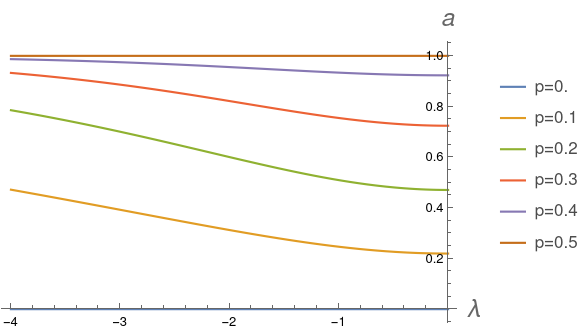
\includegraphics[width=0.6\linewidth]{maxent/figures/ContractionFactorSWAP_2D_lambda-4to0.png}
  \caption{$-4<\lambda<0$}
\end{subfigure}%
\begin{subfigure}{0.475\textwidth}
  \centering
  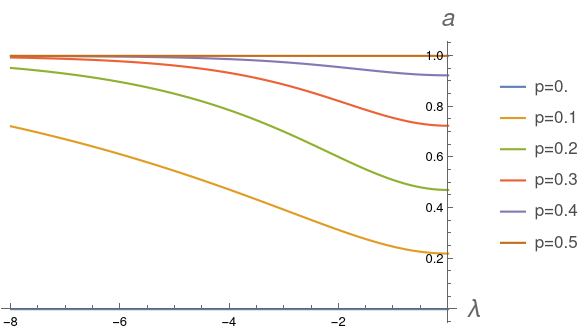
\includegraphics[width=0.6\linewidth]{maxent/figures/ContractionFactorSWAP_2D_lambda-8to0.png}
  \caption{$-8<\lambda<0$}
\end{subfigure}
\caption{Factor de compresión para diferentes valores de $p$, como función de $\lambda$. Notar el límite $\lambda\rightarrow \infty$}
\label{fig:SWAPFactorP}
\end{figure}
\begin{figure}[h!]
\centering
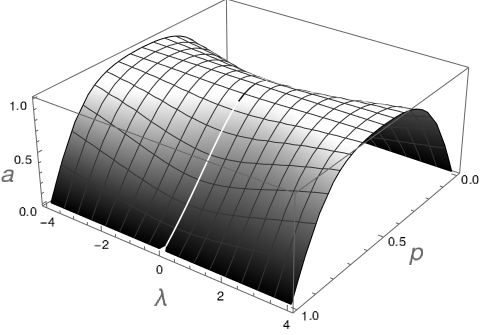
\includegraphics[width=0.6\linewidth]{maxent/figures/ContractionFactorSWAP_3D_lambda-4to4.png}
\caption{Superficie del factor de compresión como función del multiplicador de Lagrange y del parámetro de probabilidad asociado a la aplicación de grano grueso. \notaAd{Parece haber una discontinuidad en $\lambda=0$ que valdría la pena estudiar}}
\label{fig:SWAPFactorSup}
\end{figure}
Esto puede comprobarse en los resultados numéricos mostrados en la figura \ref{fig:factornnum}.
\begin{figure}[h!]
\centering
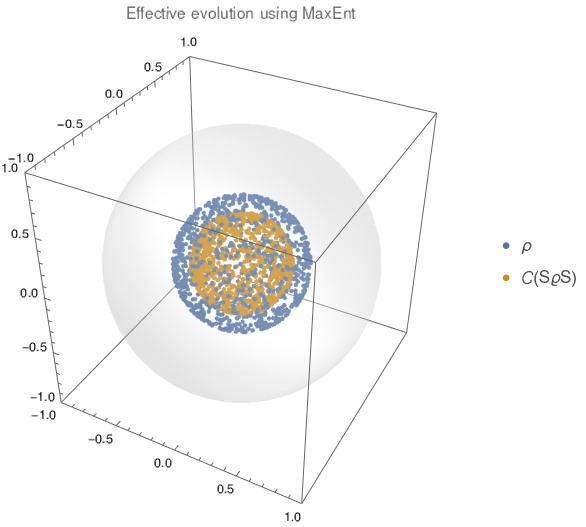
\includegraphics[width=0.6\linewidth]{maxent/figures/MaxEnt_SWAP_t0vst1_n=5000_z=0.5_p=0.3_beta=150_delta=0.6.png}
\caption{Apreciación del factor de compresión \notaAd{aquí está bueno comparar la diferencia radial numérica con el factor analítico}}
\label{fig:factornnum}
\end{figure}

Como el factor de compresión depende de $\lambda$, la dinámica no es lineal. Las operaciones cuánticas de un qubit se traducen como aplicaciones afines en la esfera de Bloch. Si quisiéramos ver el proceso asociado al $textsc{SWAP}$ subyacente como una transformación de la forma
\begin{equation*}
  \vec{r}\rightarrow M\vec{r}+\vec{c}
\end{equation*}
en la que $\vec{c}=0$, y $M=OS$ con $O=\Id$ y $S=a(\vec{r})\Id$, de tal forma que
\begin{equation*}
  \vec{r}\rightarrow a(\vec{r})\vec{r}
\end{equation*}
nos daríamos cuenta que la transformación no es afín, y por esto, el proceso no puede ser descrito a través del formalismo de las operaciones cuánticas (no tiene representación en operadores de Kraus). \cite{Chuang}.
\subsubsection{Caso $p=\frac{1}{2}$}

Aunque es posible repetir todas las cuentas desde la contrucción del estado de máxima entropía, haciendo $p=\frac{1}{2}$, basta con ver que el factor (\eqref{eq:SWAPFactor}) es $1$ en dicho caso. Así, todos los estado gruesos son puntos fijos bajo una evolución subyacente SWAP con aplicación de grano grueso con parámetro $p=\frac{1}{2}$.

\subsection{Extensión a $t$}
Siendo \textsc{SWAP} un operador unitario, anteriormente se denotó el estado inicial y final como $\varrho(0)$ y $\varrho(1)$, de acuerdo a lo establecido en la ecuación (\ref{eq:TimeDepenenceUnitary}). Para extender los resultados a un tiempo arbitrario en el intervalo $[0,1]$, es necesaria una expresión analítica del operador. El operador SWAP deja intactos a los estados $\ket{00}$ y $\ket{11}$, e intercambia $\ket{01}$ con $\ket{1,0}$. De esto, el operador también dejará invariantes (hasta un factor) a los estados $\ket{+_{2}}=\frac{\ket{01}+\ket{10}}{\sqrt{2}}$ y $\ket{-_{2}}\frac{\ket{01}-\ket{10}}{\sqrt{2}}$. Dados estos eigenestados (y eigenvalores), la descomposición espectral del operador es
\begin{equation}\label{eq:SWAPSpectral}
S=P(\dyad{00}+\dyad{11}+\dyad{+_{2}}-\dyad{-_{2}})P^{\dag}.
\end{equation}
donde $P$ es la matriz formada por los eigenestados del operador. Potenciando se halla que
\begin{align}\label{eq:SWAPPower}
S^{t}&=P(\dyad{00}+\dyad{11}+\dyad{+_{2}}+(-)^{t}\dyad{-_{2}})P^{\dag}\\
&=P(\dyad{00}+\dyad{11}+\dyad{+_{2}}+e^{i \pi t}\dyad{-_{2}})P^{\dag}
\end{align}
La forma matricial del operador \textsc{SWAP} a un tiempo $t$ es
\begin{equation}
S^{t}=\begin{pmatrix}
 1 & 0 & 0 & 0 \\
 0 & \frac{1}{2}(1+e^{i \pi t}) & \frac{1}{2} (1-e^{i \pi t}) & 0 \\
 0 & \frac{1}{2}(1-e^{i \pi t}) & \frac{1}{2}(1+e^{i \pi t}) & 0 \\
 0 & 0 & 0 & 1
\end{pmatrix}
\end{equation}
\notaAd{Lo anterior se ve bien porque es una función periódica en 
$t$ con periodo 1. Sinceramente aquí no sé que tanto deba detallar las cuentas, pero si se aplica la untaria $S^t$ al estado de máxima entropía, y si se pasa el resultado por la aplicación de grano grueso, el resultado es otro estado alineado en $z$. Esto seguro puede escribirse de forma elegante en notación de Dirac y pues me toca sacarlo bien. Haciendo cuentas a lo tonto uno puede hallar el factor de compresión para $t$ arbitrario:
\begin{equation}
a(\lambda,p,t)=\frac{e^{-\lambda -2 \lambda  p-i \pi  t} \left(2 \left(e^{2 \lambda }-1\right) e^{2 \lambda  p+i \pi  t}-e^{2 \lambda } (2 p-1) \left(1+e^{2 i \pi  t}\right)+(2 p-1) \left(1+e^{2 i \pi  t}\right) e^{4 \lambda  p}\right)}{4 (\sinh (\lambda )+(1-2 p) \sinh (\lambda -2 \lambda  p))}
\end{equation}
Aquí toca verificar que se recupera lo esperado para $t=0,1$. Además, toca ver si es creciente, decrececiente, y tal, para valores fijos de los otros dos parámetros. Una derivadita parcial should do the trick.
}
\newpage